
%\documentclass[mathserif]{beamer}
\documentclass[handout]{beamer}
%\usetheme{Goettingen}
%\usetheme{Warsaw}
\usetheme{Singapore}



%\usetheme{Frankfurt}
%\usetheme{Copenhagen}
%\usetheme{Szeged}
%\usetheme{Montpellier}
%\usetheme{CambridgeUS}
%\usecolortheme{}
%\setbeamercovered{transparent}
\usepackage[english, activeacute]{babel}
\usepackage[utf8]{inputenc}
\usepackage{amsmath, amssymb}
\usepackage{dsfont}
\usepackage{graphics}
\usepackage{cases}
\usepackage{graphicx}
\usepackage{pgf}
\usepackage{epsfig}
\usepackage{amssymb}
\usepackage{multirow}	
\usepackage{amstext}
\usepackage[ruled,vlined,lined]{algorithm2e}
\usepackage{amsmath}
\usepackage{epic}
\usepackage{epsfig}
\usepackage{fontenc}
\usepackage{framed,color}
\usepackage{palatino, url, multicol}
%\algsetup{indent=2em}
\newcommand{\factorial}{\ensuremath{\mbox{\sc Factorial}}}
\newcommand{\BIGOP}[1]{\mathop{\mathchoice%
{\raise-0.22em\hbox{\huge $#1$}}%
{\raise-0.05em\hbox{\Large $#1$}}{\hbox{\large $#1$}}{#1}}}
\newcommand{\bigtimes}{\BIGOP{\times}}
\vspace{-0.5cm}
\title{Natural Language Processing \\ Convolutional Neural Networks}
\vspace{-0.5cm}
\author[Felipe Bravo Márquez]{\footnotesize
%\author{\footnotesize  
 \textcolor[rgb]{0.00,0.00,1.00}{Felipe Bravo-Marquez}} 
  
 

\date{\today}

\begin{document}
\begin{frame}
\titlepage


\end{frame}



\begin{frame}{Convolutional Neural Networks}
\begin{scriptsize}
\begin{itemize}
\item Convolutional neural networks (CNNs) became very popular in the computer vision community due to its success for detecting objects (``cat'',``bicycles'') regardless of its position in the image.
\item They identify indicative local predictors in a structure (e.g., images, sentences).
\item These predictors are combined to produce a fixed size vector representation for the structure.
\item When used in NLP, the network captures the n-grams that are most informative for the target predictive task.
\item For sentiment classification, these local aspects correspond to n-grams conveying sentiment (e.g., not bad, very good).
\item The fundamental idea of CNNs \cite{lecun1998gradient}  is  to  consider  feature extraction and classification as one jointly trained task. 

\end{itemize}
\end{scriptsize}
\end{frame}

\begin{frame}{Basic Convolution  + Pooling}
\begin{scriptsize}
\begin{itemize}
\item Sentences are usually modelled as sequences of word embeddings.
\item The CNN applies  nonlinear (learned) functions or ``filters'' mapping windows of $k$ words into scalar values.
\item Several filters can be applied, resulting in an $l$-dimensional vector (one dimension per filter).
\item The filters capture relevant properties of the words in the window.
\item These filters correspond to the ``convolution layer'' of the network.
\end{itemize}
\end{scriptsize}
\end{frame}

\begin{frame}{Basic Convolution  + Pooling}
\begin{scriptsize}
\begin{itemize}
\item The ``pooling'' layer is used
to combine the vectors resulting from the different windows into a single $l$-dimensional vector.
\item This is done by taking the max or the average value observed in each of the dimensions over the different windows.
\item The goal is to capture the most important ``features'' in the sentence, regardless of the position.
\item The resulting $l$-dimensional vector is then fed further into a network that is used for prediction (e.g., softmax).
\item The gradients are propagated back from the network's loss tuning the parameters of the filter.
\item The filters learn to highlight the aspects of the data (n-grams) that are important for the target task. 
\end{itemize}
\end{scriptsize}
\end{frame}



\begin{frame}{Basic Convolution  + Pooling}
  \begin{figure}[h]
        	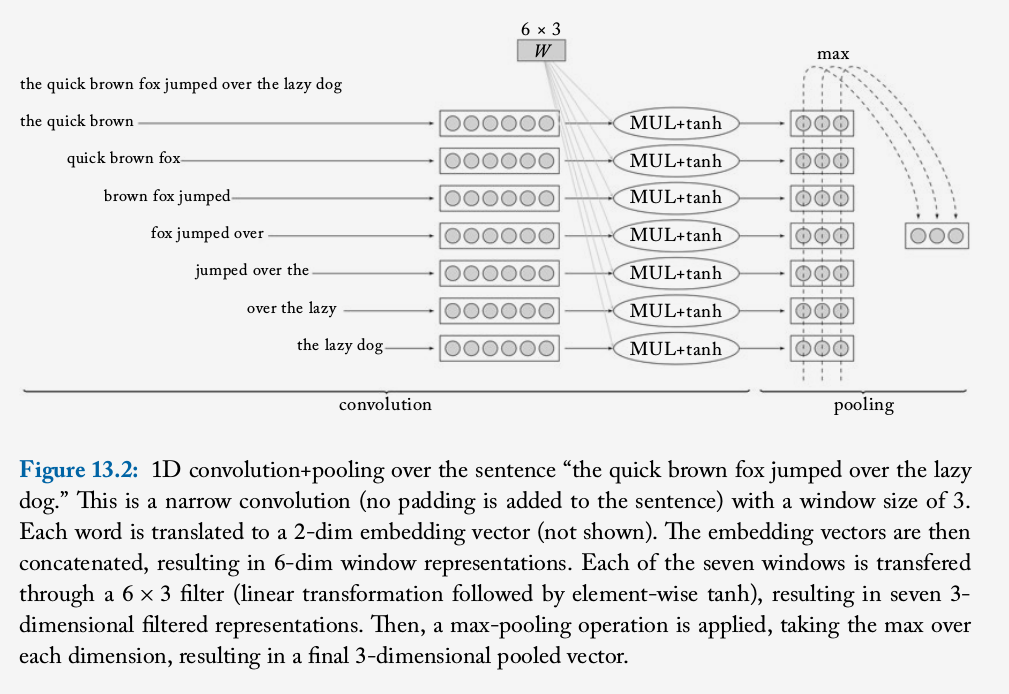
\includegraphics[scale = 0.28]{pics/CNN.png}
        \end{figure}
 \footnotemark{Source: \cite{goldberg2016primer}}   
\end{frame}



\begin{frame}{1D Convolutions over Text}
\begin{scriptsize}
\begin{itemize}
\item We focus on the one-dimensional convolution operation\footnote{1D here refers to a convolution operating over 1-dimensional inputs such as sequences, as opposed to 2D convolutions which
are applied to images.}.
\item Consider a sequence of words $w_{1:n}=w_1 ,\dots,w_n$ each with their corresponding $d_{emb}$ dimensional word embedding $E_{[w_i]}=\vec{w}_{i}$.
\item A 1D convolution of width $k$ works by moving a sliding-window of size $k$ over the sentence, and applying the same filter to each window
in the sequence.
\item A filter is a dot-product with a weight vector $\vec{u}$ , which is often followed by a nonlinear activation function.
\end{itemize}
\end{scriptsize}
\end{frame}

\begin{frame}{1D Convolutions over Text}
\begin{scriptsize}
\begin{itemize}
\item Define the operator $\oplus (w_{i:i+k-1})$ to be the concatenation of the vectors $\vec{w}_{i}, \dots, \vec{w}_{i+k-1}$.
\item The concatenated vector of the $i$-th window is $\vec{x}_{i}=\oplus (w_{i:i+k-1}) = [\vec{w}_{i};\vec{w}_{i+1};\dots;\vec{w}_{i+k-1}]$, $x_{i} \in \mathcal{R}^{k \cdot d_{emb}}$.
\item We then apply the filter to each window vector resulting in scalar values $p_{i} =  g(\vec{x}_{i} \cdot \vec{u})$. ($p_{i} \in \mathcal{R}$)
\item It is customary to use $l$ different filters, $\vec{u}_1,\dots, \vec{u}_l$, which can be arranged into a matrix $U$, and a bias vector $\vec{b}$ is often added: $\vec{p}_{i}=g(\vec{x}_{i}\cdot U +\vec{b})$.

\item Each vector $\vec{p}_i$ is a collection of $l$ values that represent (or summarise) the $i$-th window ($\vec{p}_{i} \in \mathcal{R}^l$). 
\item Ideally, each dimension captures a different kind of indicative information.

\end{itemize}
\end{scriptsize}
\end{frame}


\begin{frame}{Narrow vs. Wide Convolutions}
\begin{scriptsize}
\begin{itemize}
\item How many vectors $\vec{p}_i$ do we have?
\item For a sentence of length $n$ with a window of size $k$, there are $n - k + 1$ positions in which to start the sequence. 
\item We get $n - k + 1$ vectors $\vec{p}_{1:n-k+1}$. 
\item This approach is called \textbf{narrow convolution}.
\item An alternative is to pad the sentence with $k - 1$ padding-words to each side, resulting in $n+k+1$ vectors $\vec{p}_{1:n+k+1}$. 
\item This is called a \textbf{wide convolution}.
\end{itemize}
\end{scriptsize}
\end{frame}


\begin{frame}{1D Convolutions over Text}
\begin{scriptsize}
\begin{itemize}
\item The main idea behind the convolution layer is to apply the same parameterised function over all $k$-grams in the sequence.
\item This creates a sequence of $m$ vectors, each representing
a particular $k$-gram in the sequence.
\item The representation is sensitive to the identity and order of the words within a $k$-gram.
\item However, the same representation will be extracted for a $k$-gram regardless of its position within the sequence.
\end{itemize}
\end{scriptsize}
\end{frame}



\begin{frame}{Vector Pooling}
\begin{scriptsize}
\begin{itemize}
\item Applying the convolution over the text results in $m$ vectors $\vec{p}_{1:m}$, each $\vec{p}_i \in \mathcal{R}^l$.
\item These vectors are then combined (pooled) into a single vector $c \in \mathcal{R}^l$ representing the entire sequence.
\item Max pooling: this operator takes the maximum value across each dimension (most common pooling operation).
\begin{displaymath}
c_[j]= \max_{1< i \leq m} p_{i[j]} \quad \forall j \in [1,l]
\end{displaymath}

\item Average Pooling (second most common): takes the average value of each index:
\begin{displaymath}
c = \frac{1}{m} \sum_{i=1}^{m}p_i
\end{displaymath}

\item Ideally, the vector $c$ will capture the essence of the important information in the sequence. 

\end{itemize}
\end{scriptsize}
\end{frame}



\begin{frame}{Vector Pooling}
\begin{scriptsize}
\begin{itemize}
\item The nature of the important information that needs to be encoded in the vector $c$ is task dependent. 
\item If we are performing sentiment classification, the essence are informative ngrams that indicate
sentiment.
\item If we are performing topic-classification, the essence are informative $n$-grams that indicate a particular topic.

\item During training, the vector $c$ is fed into downstream network layers (i.e., an MLP), culminating in an output layer which is used for prediction.
\item The training procedure of the network calculates the loss with respect to the prediction task, and the error gradients are propagated all the way back through the pooling and convolution layers, as well as the embedding layers. 
\item The training process tunes the convolution matrix $U$, the bias vector $\vec{b}$, the downstream network, and
potentially also the embeddings matrix $E$\footnote{While some people leave the embedding layer fixed during training, others allow the parameters to change.}  such that the vector $c$ resulting from the convolution
and pooling process indeed encodes information relevant to the task at hand.
\end{itemize}
\end{scriptsize}
\end{frame}



\begin{frame}{Twitter Sentiment Classification with CNN}
\begin{scriptsize}
\begin{itemize}
\item A convolutional neural network architecture for Twitter sentiment classification is developed in \cite{Severyn2015}.
\item  Each tweet is represented as a matrix whose columns correspond to the words in the tweet, preserving the order in which they occur.
\item  The words are represented by dense vectors or embeddings trained from a large corpus of unlabelled tweets using word2vec.
\item  The network is formed by the following layers: an input layer with the given tweet matrix, a  single  convolutional layer, a rectified linear activation function, a max pooling layer, and a soft-max classification layer.
\end{itemize}
\end{scriptsize}
\end{frame}


\begin{frame}{Twitter Sentiment Classification with CNN}
\begin{scriptsize}
\begin{itemize}
\item  The weights of the neural network are pre-trained using emoticon-annotated data, and then trained with the hand-annotated tweets from the SemEval competition.
\item   Experimental results show that the pre-training phase allows for a proper initialisation of the network's weights, and hence, has a positive impact on classification accuracy. 
\end{itemize}
  \begin{figure}[h]
        	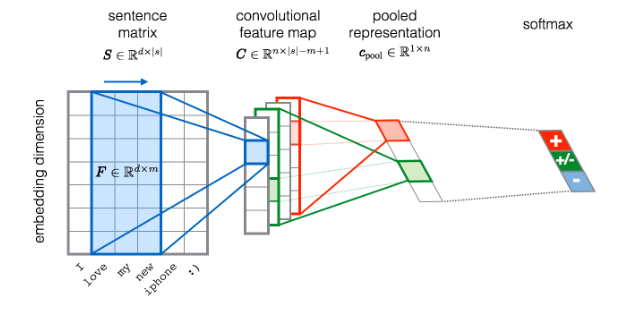
\includegraphics[scale = 0.45]{pics/cnn-twitter.png}
        \end{figure}
\end{scriptsize}
\end{frame}




\begin{frame}{Very Deep Convolutional Networks for Text Classification}
\begin{scriptsize}
\begin{itemize}
\item CNNs architectures for NLP are rather shallow in comparison to the deep convolutional networks which have pushed the state-of-the-art in computer vision.
\item A new architecture (VDCNN) for text processing which operates directly at the character level and uses only small convolutions and pooling operations is proposed in \cite{conneau2017very}.

\item Character-level embeddings are used instead of word-embeddings.

\item Characters are the lowest atomic representation of text. 

\item The performance of this model increases with depth: using up to 29 convolutional layers, authors report improvements over the state-of-the-art on several public text classification tasks. 

\item Most notorious improvements are achieved on large datasets.

\item First paper showing the the benefits  of  depth architectures for NLP.
\end{itemize}
\end{scriptsize}
\end{frame}






\begin{frame}{Very Deep Convolutional Networks for Text Classification}

  \begin{figure}[h]
        	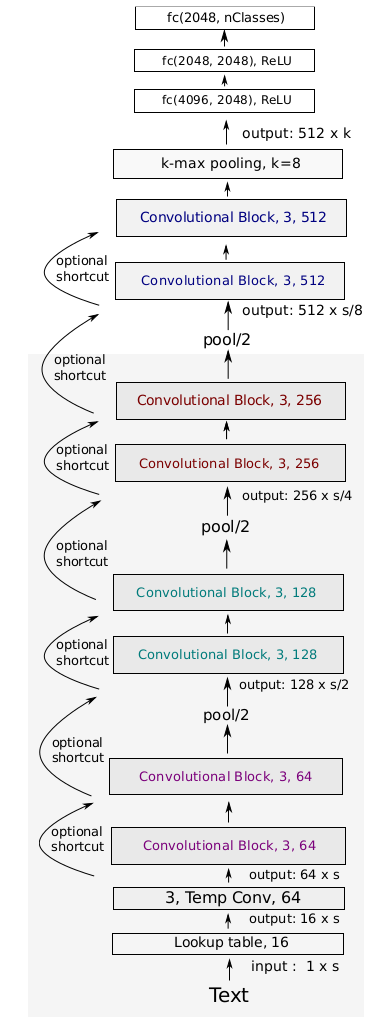
\includegraphics[scale = 0.2]{pics/VDCNN.png}
        \end{figure}

\end{frame}





\begin{frame}
\frametitle{Questions?}
%\vspace{1.5cm}
\begin{center}\LARGE Thanks for your Attention!\\ \end{center}



\end{frame}

\begin{frame}[allowframebreaks]\scriptsize
\frametitle{References}
\bibliography{bio}
\bibliographystyle{apalike}
%\bibliographystyle{flexbib}
\end{frame}  


%%%%%%%%%%%%%%%%%%%%%%%%%%%

\end{document}
